\documentclass{standalone}
\usepackage{tikz}
\usetikzlibrary{patterns, positioning}


\begin{document}
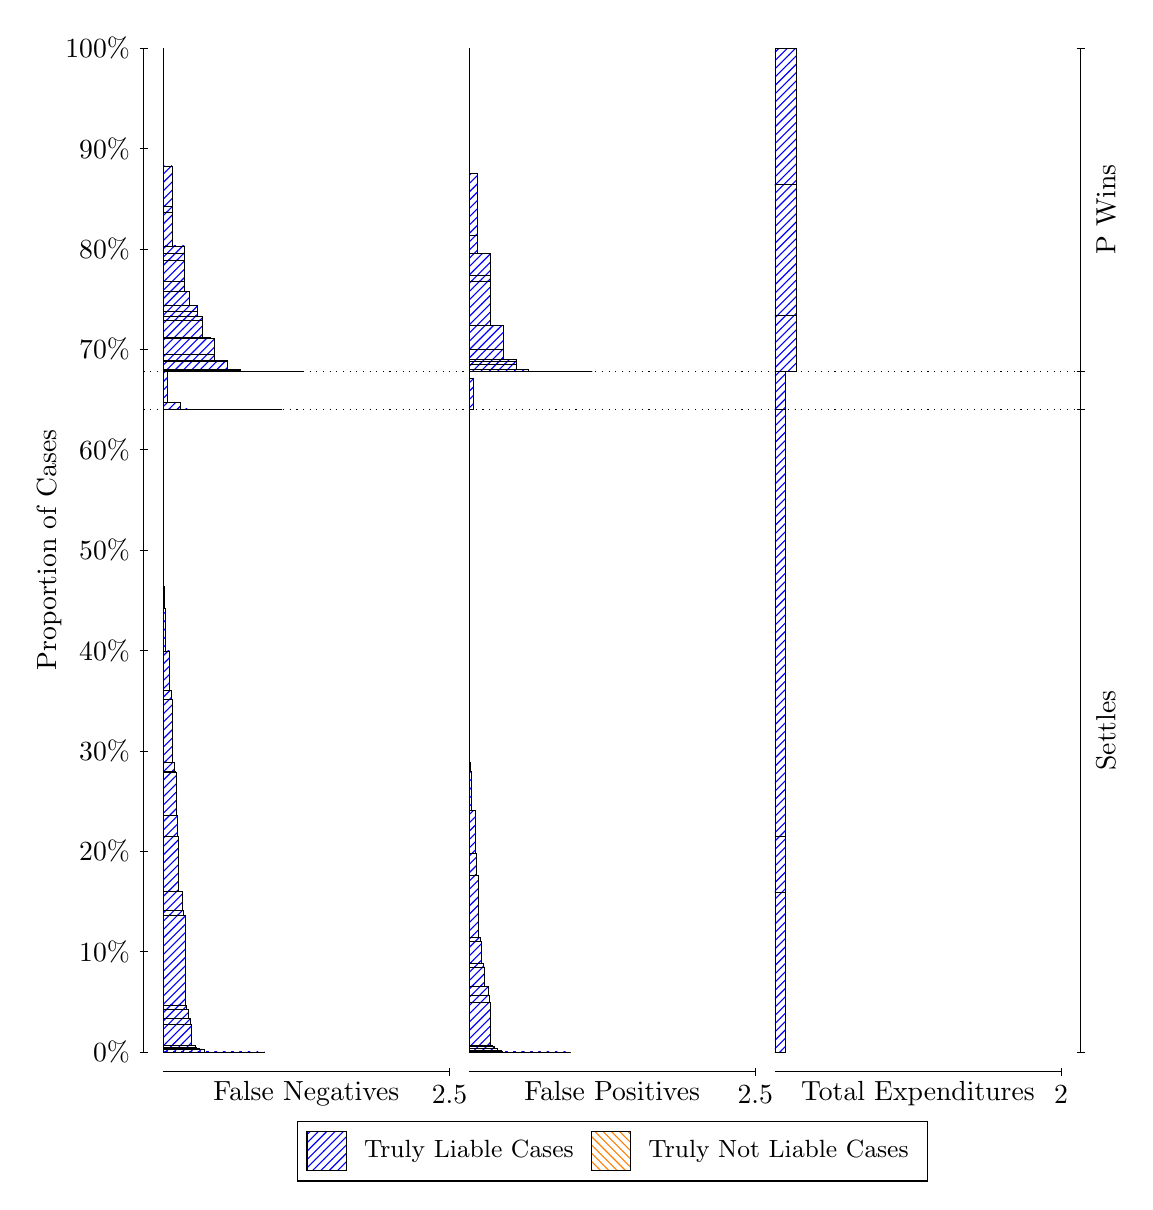
\begin{tikzpicture}
\draw[black, very thin] (1.5,1.75) -- (1.5,14.5);
\node[rotate=90, text=black, anchor=center] at (0.3, 8.125) {Proportion of Cases};
\draw[black, very thin] (1.45,1.75) -- (1.55,1.75);
\node[text=black, anchor=east] at (1.45, 1.75) {0\%};
\draw[black, very thin] (1.45,3.025) -- (1.55,3.025);
\node[text=black, anchor=east] at (1.45, 3.025) {10\%};
\draw[black, very thin] (1.45,4.3) -- (1.55,4.3);
\node[text=black, anchor=east] at (1.45, 4.3) {20\%};
\draw[black, very thin] (1.45,5.575) -- (1.55,5.575);
\node[text=black, anchor=east] at (1.45, 5.575) {30\%};
\draw[black, very thin] (1.45,6.85) -- (1.55,6.85);
\node[text=black, anchor=east] at (1.45, 6.85) {40\%};
\draw[black, very thin] (1.45,8.125) -- (1.55,8.125);
\node[text=black, anchor=east] at (1.45, 8.125) {50\%};
\draw[black, very thin] (1.45,9.4) -- (1.55,9.4);
\node[text=black, anchor=east] at (1.45, 9.4) {60\%};
\draw[black, very thin] (1.45,10.675) -- (1.55,10.675);
\node[text=black, anchor=east] at (1.45, 10.675) {70\%};
\draw[black, very thin] (1.45,11.95) -- (1.55,11.95);
\node[text=black, anchor=east] at (1.45, 11.95) {80\%};
\draw[black, very thin] (1.45,13.225) -- (1.55,13.225);
\node[text=black, anchor=east] at (1.45, 13.225) {90\%};
\draw[black, very thin] (1.45,14.5) -- (1.55,14.5);
\node[text=black, anchor=east] at (1.45, 14.5) {100\%};

\draw[black, very thin] (13.4,1.75) -- (13.4,14.5);
\draw[black, very thin] (13.35,1.75) -- (13.45,1.75);
\node[anchor=west] at (13.35, 1.75) {};
\draw[black, very thin] (13.35,9.9125) -- (13.45,9.9125);
\node[anchor=west] at (13.35, 9.9125) {};
\draw[black, very thin] (13.35,10.394) -- (13.45,10.394);
\node[anchor=west] at (13.35, 10.394) {};
\draw[black, very thin] (13.35,14.5) -- (13.45,14.5);
\node[anchor=west] at (13.35, 14.5) {};

\draw[black, very thin, pattern color=blue, pattern=north east lines] (1.75,1.75) rectangle (3.0398,1.75);
\draw[black, very thin, pattern color=blue, pattern=north east lines] (1.75,1.75) rectangle (2.8945,1.75);
\draw[black, very thin, pattern color=blue, pattern=north east lines] (1.75,1.75) rectangle (2.8784,1.75);
\draw[black, very thin, pattern color=blue, pattern=north east lines] (1.75,1.75) rectangle (2.7492,1.75);
\draw[black, very thin, pattern color=blue, pattern=north east lines] (1.75,1.75) rectangle (2.733,1.75);
\draw[black, very thin, pattern color=blue, pattern=north east lines] (1.75,1.75) rectangle (2.7169,1.75);
\draw[black, very thin, pattern color=blue, pattern=north east lines] (1.75,1.75) rectangle (2.6765,1.75);
\draw[black, very thin, pattern color=blue, pattern=north east lines] (1.75,1.75) rectangle (2.5877,1.75);
\draw[black, very thin, pattern color=blue, pattern=north east lines] (1.75,1.75) rectangle (2.5715,1.75);
\draw[black, very thin, pattern color=blue, pattern=north east lines] (1.75,1.75) rectangle (2.5554,1.75);
\draw[black, very thin, pattern color=blue, pattern=north east lines] (1.75,1.75) rectangle (2.5312,1.75);
\draw[black, very thin, pattern color=blue, pattern=north east lines] (1.75,1.75) rectangle (2.515,1.75);
\draw[black, very thin, pattern color=blue, pattern=north east lines] (1.75,1.75) rectangle (2.4262,1.7505);
\draw[black, very thin, pattern color=blue, pattern=north east lines] (1.75,1.7505) rectangle (2.4101,1.7506);
\draw[black, very thin, pattern color=blue, pattern=north east lines] (1.75,1.7506) rectangle (2.3939,1.7507);
\draw[black, very thin, pattern color=blue, pattern=north east lines] (1.75,1.7507) rectangle (2.3858,1.7507);
\draw[black, very thin, pattern color=blue, pattern=north east lines] (1.75,1.7507) rectangle (2.3697,1.7508);
\draw[black, very thin, pattern color=blue, pattern=north east lines] (1.75,1.7508) rectangle (2.3535,1.7508);
\draw[black, very thin, pattern color=blue, pattern=north east lines] (1.75,1.7508) rectangle (2.3132,1.7519);
\draw[black, very thin, pattern color=blue, pattern=north east lines] (1.75,1.7519) rectangle (2.2647,1.7781);
\draw[black, very thin, pattern color=blue, pattern=north east lines] (1.75,1.7781) rectangle (2.2486,1.7835);
\draw[black, very thin, pattern color=blue, pattern=north east lines] (1.75,1.7835) rectangle (2.2324,1.7892);
\draw[black, very thin, pattern color=blue, pattern=north east lines] (1.75,1.7892) rectangle (2.2244,1.7894);
\draw[black, very thin, pattern color=blue, pattern=north east lines] (1.75,1.7894) rectangle (2.2082,1.7944);
\draw[black, very thin, pattern color=blue, pattern=north east lines] (1.75,1.7944) rectangle (2.1921,1.7946);
\draw[black, very thin, pattern color=blue, pattern=north east lines] (1.75,1.7946) rectangle (2.1678,1.8049);
\draw[black, very thin, pattern color=blue, pattern=north east lines] (1.75,1.8049) rectangle (2.1517,1.8344);
\draw[black, very thin, pattern color=blue, pattern=north east lines] (1.75,1.8344) rectangle (2.1032,2.0985);
\draw[black, very thin, pattern color=blue, pattern=north east lines] (1.75,2.0985) rectangle (2.0871,2.1723);
\draw[black, very thin, pattern color=blue, pattern=north east lines] (1.75,2.1723) rectangle (2.0709,2.2912);
\draw[black, very thin, pattern color=blue, pattern=north east lines] (1.75,2.2912) rectangle (2.0629,2.2936);
\draw[black, very thin, pattern color=blue, pattern=north east lines] (1.75,2.2936) rectangle (2.0467,2.3467);
\draw[black, very thin, pattern color=blue, pattern=north east lines] (1.75,2.3467) rectangle (2.0306,2.3491);
\draw[black, very thin, pattern color=blue, pattern=north east lines] (1.75,2.3491) rectangle (2.0225,3.4906);
\draw[black, very thin, pattern color=blue, pattern=north east lines] (1.75,3.4906) rectangle (2.0064,3.5515);
\draw[black, very thin, pattern color=blue, pattern=north east lines] (1.75,3.5515) rectangle (1.9902,3.7953);
\draw[black, very thin, pattern color=blue, pattern=north east lines] (1.75,3.7953) rectangle (1.9418,4.4853);
\draw[black, very thin, pattern color=blue, pattern=north east lines] (1.75,4.4853) rectangle (1.9256,4.7548);
\draw[black, very thin, pattern color=blue, pattern=north east lines] (1.75,4.7548) rectangle (1.9095,5.3074);
\draw[black, very thin, pattern color=blue, pattern=north east lines] (1.75,5.3074) rectangle (1.9014,5.3131);
\draw[black, very thin, pattern color=blue, pattern=north east lines] (1.75,5.3131) rectangle (1.8852,5.4296);
\draw[black, very thin, pattern color=blue, pattern=north east lines] (1.75,5.4296) rectangle (1.8691,5.4353);
\draw[black, very thin, pattern color=blue, pattern=north east lines] (1.75,5.4353) rectangle (1.861,6.2277);
\draw[black, very thin, pattern color=blue, pattern=north east lines] (1.75,6.2277) rectangle (1.8449,6.3457);
\draw[black, very thin, pattern color=blue, pattern=north east lines] (1.75,6.3457) rectangle (1.8287,6.8434);
\draw[black, very thin, pattern color=blue, pattern=north east lines] (1.75,6.8434) rectangle (1.7803,7.3894);
\draw[black, very thin, pattern color=blue, pattern=north east lines] (1.75,7.3894) rectangle (1.7641,7.6622);
\draw[black, very thin, pattern color=orange, pattern=north west lines] (1.75,7.6622) rectangle (1.75,7.6622);
\draw[black, very thin, pattern color=blue, pattern=north east lines] (1.75,7.6622) rectangle (1.75,9.9125);
\draw[black, very thin, pattern color=blue, pattern=north east lines] (1.75,9.9125) rectangle (3.2578,9.9125);
\draw[black, very thin, pattern color=blue, pattern=north east lines] (1.75,9.9125) rectangle (3.0964,9.9125);
\draw[black, very thin, pattern color=blue, pattern=north east lines] (1.75,9.9125) rectangle (2.9349,9.9125);
\draw[black, very thin, pattern color=blue, pattern=north east lines] (1.75,9.9125) rectangle (2.7734,9.9125);
\draw[black, very thin, pattern color=blue, pattern=north east lines] (1.75,9.9125) rectangle (2.6119,9.9125);
\draw[black, very thin, pattern color=blue, pattern=north east lines] (1.75,9.9125) rectangle (2.4504,9.9125);
\draw[black, very thin, pattern color=blue, pattern=north east lines] (1.75,9.9125) rectangle (2.2889,9.9126);
\draw[black, very thin, pattern color=blue, pattern=north east lines] (1.75,9.9126) rectangle (2.1275,9.9173);
\draw[black, very thin, pattern color=blue, pattern=north east lines] (1.75,9.9173) rectangle (1.966,10.003);
\draw[black, very thin, pattern color=blue, pattern=north east lines] (1.75,10.003) rectangle (1.8045,10.394);
\draw[black, very thin, pattern color=orange, pattern=north west lines] (1.75,10.394) rectangle (1.75,10.394);
\draw[black, very thin, pattern color=blue, pattern=north east lines] (1.75,10.394) rectangle (3.5303,10.394);
\draw[black, very thin, pattern color=blue, pattern=north east lines] (1.75,10.394) rectangle (3.3689,10.394);
\draw[black, very thin, pattern color=blue, pattern=north east lines] (1.75,10.394) rectangle (3.2074,10.394);
\draw[black, very thin, pattern color=blue, pattern=north east lines] (1.75,10.394) rectangle (3.1509,10.394);
\draw[black, very thin, pattern color=blue, pattern=north east lines] (1.75,10.394) rectangle (3.0459,10.394);
\draw[black, very thin, pattern color=blue, pattern=north east lines] (1.75,10.394) rectangle (2.9894,10.394);
\draw[black, very thin, pattern color=blue, pattern=north east lines] (1.75,10.394) rectangle (2.9894,10.394);
\draw[black, very thin, pattern color=blue, pattern=north east lines] (1.75,10.394) rectangle (2.8844,10.396);
\draw[black, very thin, pattern color=blue, pattern=north east lines] (1.75,10.396) rectangle (2.8844,10.397);
\draw[black, very thin, pattern color=blue, pattern=north east lines] (1.75,10.397) rectangle (2.8279,10.397);
\draw[black, very thin, pattern color=blue, pattern=north east lines] (1.75,10.397) rectangle (2.7229,10.408);
\draw[black, very thin, pattern color=blue, pattern=north east lines] (1.75,10.408) rectangle (2.7229,10.423);
\draw[black, very thin, pattern color=blue, pattern=north east lines] (1.75,10.423) rectangle (2.6664,10.423);
\draw[black, very thin, pattern color=blue, pattern=north east lines] (1.75,10.423) rectangle (2.5614,10.521);
\draw[black, very thin, pattern color=blue, pattern=north east lines] (1.75,10.521) rectangle (2.5614,10.538);
\draw[black, very thin, pattern color=blue, pattern=north east lines] (1.75,10.538) rectangle (2.5049,10.538);
\draw[black, very thin, pattern color=blue, pattern=north east lines] (1.75,10.538) rectangle (2.5049,10.538);
\draw[black, very thin, pattern color=blue, pattern=north east lines] (1.75,10.538) rectangle (2.4,10.608);
\draw[black, very thin, pattern color=blue, pattern=north east lines] (1.75,10.608) rectangle (2.4,10.812);
\draw[black, very thin, pattern color=blue, pattern=north east lines] (1.75,10.812) rectangle (2.3434,10.816);
\draw[black, very thin, pattern color=blue, pattern=north east lines] (1.75,10.816) rectangle (2.3434,10.823);
\draw[black, very thin, pattern color=blue, pattern=north east lines] (1.75,10.823) rectangle (2.3434,10.824);
\draw[black, very thin, pattern color=blue, pattern=north east lines] (1.75,10.824) rectangle (2.2385,10.829);
\draw[black, very thin, pattern color=blue, pattern=north east lines] (1.75,10.829) rectangle (2.2385,11.046);
\draw[black, very thin, pattern color=blue, pattern=north east lines] (1.75,11.046) rectangle (2.2385,11.098);
\draw[black, very thin, pattern color=blue, pattern=north east lines] (1.75,11.098) rectangle (2.182,11.099);
\draw[black, very thin, pattern color=blue, pattern=north east lines] (1.75,11.099) rectangle (2.182,11.16);
\draw[black, very thin, pattern color=blue, pattern=north east lines] (1.75,11.16) rectangle (2.182,11.233);
\draw[black, very thin, pattern color=blue, pattern=north east lines] (1.75,11.233) rectangle (2.077,11.407);
\draw[black, very thin, pattern color=blue, pattern=north east lines] (1.75,11.407) rectangle (2.0205,11.536);
\draw[black, very thin, pattern color=blue, pattern=north east lines] (1.75,11.536) rectangle (2.0205,11.81);
\draw[black, very thin, pattern color=blue, pattern=north east lines] (1.75,11.81) rectangle (2.0205,11.888);
\draw[black, very thin, pattern color=blue, pattern=north east lines] (1.75,11.888) rectangle (2.0205,11.986);
\draw[black, very thin, pattern color=blue, pattern=north east lines] (1.75,11.986) rectangle (1.9155,11.988);
\draw[black, very thin, pattern color=blue, pattern=north east lines] (1.75,11.988) rectangle (1.9155,11.988);
\draw[black, very thin, pattern color=blue, pattern=north east lines] (1.75,11.988) rectangle (1.859,12.419);
\draw[black, very thin, pattern color=blue, pattern=north east lines] (1.75,12.419) rectangle (1.859,12.495);
\draw[black, very thin, pattern color=blue, pattern=north east lines] (1.75,12.495) rectangle (1.859,13.004);
\draw[black, very thin, pattern color=blue, pattern=north east lines] (1.75,13.004) rectangle (1.754,13.004);
\draw[black, very thin, pattern color=blue, pattern=north east lines] (1.75,13.004) rectangle (1.754,13.004);
\draw[black, very thin, pattern color=orange, pattern=north west lines] (1.75,13.004) rectangle (1.75,13.004);
\draw[black, very thin, pattern color=blue, pattern=north east lines] (1.75,13.004) rectangle (1.75,14.5);
\draw[black, very thin, pattern color=orange, pattern=north west lines] (5.6333,1.75) rectangle (6.9232,1.75);
\draw[black, very thin, pattern color=blue, pattern=north east lines] (5.6333,1.75) rectangle (6.9232,1.75);
\draw[black, very thin, pattern color=orange, pattern=north west lines] (5.6333,1.75) rectangle (6.7778,1.75);
\draw[black, very thin, pattern color=blue, pattern=north east lines] (5.6333,1.75) rectangle (6.7778,1.75);
\draw[black, very thin, pattern color=blue, pattern=north east lines] (5.6333,1.75) rectangle (6.7617,1.75);
\draw[black, very thin, pattern color=orange, pattern=north west lines] (5.6333,1.75) rectangle (6.6325,1.75);
\draw[black, very thin, pattern color=blue, pattern=north east lines] (5.6333,1.75) rectangle (6.6325,1.75);
\draw[black, very thin, pattern color=blue, pattern=north east lines] (5.6333,1.75) rectangle (6.6164,1.75);
\draw[black, very thin, pattern color=blue, pattern=north east lines] (5.6333,1.75) rectangle (6.6002,1.75);
\draw[black, very thin, pattern color=orange, pattern=north west lines] (5.6333,1.75) rectangle (6.5598,1.75);
\draw[black, very thin, pattern color=blue, pattern=north east lines] (5.6333,1.75) rectangle (6.5598,1.75);
\draw[black, very thin, pattern color=blue, pattern=north east lines] (5.6333,1.75) rectangle (6.471,1.75);
\draw[black, very thin, pattern color=blue, pattern=north east lines] (5.6333,1.75) rectangle (6.4549,1.75);
\draw[black, very thin, pattern color=blue, pattern=north east lines] (5.6333,1.75) rectangle (6.4387,1.75);
\draw[black, very thin, pattern color=orange, pattern=north west lines] (5.6333,1.75) rectangle (6.4145,1.75);
\draw[black, very thin, pattern color=blue, pattern=north east lines] (5.6333,1.75) rectangle (6.4145,1.75);
\draw[black, very thin, pattern color=blue, pattern=north east lines] (5.6333,1.75) rectangle (6.3984,1.75);
\draw[black, very thin, pattern color=blue, pattern=north east lines] (5.6333,1.75) rectangle (6.3095,1.75);
\draw[black, very thin, pattern color=blue, pattern=north east lines] (5.6333,1.75) rectangle (6.2934,1.75);
\draw[black, very thin, pattern color=blue, pattern=north east lines] (5.6333,1.75) rectangle (6.2772,1.75);
\draw[black, very thin, pattern color=orange, pattern=north west lines] (5.6333,1.75) rectangle (6.2692,1.75);
\draw[black, very thin, pattern color=blue, pattern=north east lines] (5.6333,1.75) rectangle (6.2692,1.75);
\draw[black, very thin, pattern color=blue, pattern=north east lines] (5.6333,1.75) rectangle (6.253,1.75);
\draw[black, very thin, pattern color=blue, pattern=north east lines] (5.6333,1.75) rectangle (6.2369,1.75);
\draw[black, very thin, pattern color=orange, pattern=north west lines] (5.6333,1.75) rectangle (6.1965,1.75);
\draw[black, very thin, pattern color=blue, pattern=north east lines] (5.6333,1.75) rectangle (6.1965,1.7501);
\draw[black, very thin, pattern color=blue, pattern=north east lines] (5.6333,1.7501) rectangle (6.1481,1.7506);
\draw[black, very thin, pattern color=blue, pattern=north east lines] (5.6333,1.7506) rectangle (6.1319,1.7507);
\draw[black, very thin, pattern color=blue, pattern=north east lines] (5.6333,1.7507) rectangle (6.1158,1.7513);
\draw[black, very thin, pattern color=blue, pattern=north east lines] (5.6333,1.7513) rectangle (6.1077,1.7513);
\draw[black, very thin, pattern color=blue, pattern=north east lines] (5.6333,1.7513) rectangle (6.0915,1.7513);
\draw[black, very thin, pattern color=blue, pattern=north east lines] (5.6333,1.7513) rectangle (6.0754,1.7514);
\draw[black, very thin, pattern color=orange, pattern=north west lines] (5.6333,1.7514) rectangle (6.0512,1.7514);
\draw[black, very thin, pattern color=blue, pattern=north east lines] (5.6333,1.7514) rectangle (6.0512,1.7627);
\draw[black, very thin, pattern color=blue, pattern=north east lines] (5.6333,1.7627) rectangle (6.035,1.7692);
\draw[black, very thin, pattern color=blue, pattern=north east lines] (5.6333,1.7692) rectangle (5.9866,1.7949);
\draw[black, very thin, pattern color=blue, pattern=north east lines] (5.6333,1.7949) rectangle (5.9704,1.7998);
\draw[black, very thin, pattern color=blue, pattern=north east lines] (5.6333,1.7998) rectangle (5.9543,1.826);
\draw[black, very thin, pattern color=blue, pattern=north east lines] (5.6333,1.826) rectangle (5.9462,1.8262);
\draw[black, very thin, pattern color=blue, pattern=north east lines] (5.6333,1.8262) rectangle (5.9301,1.8311);
\draw[black, very thin, pattern color=blue, pattern=north east lines] (5.6333,1.8311) rectangle (5.9139,1.8313);
\draw[black, very thin, pattern color=orange, pattern=north west lines] (5.6333,1.8313) rectangle (5.9058,1.8313);
\draw[black, very thin, pattern color=blue, pattern=north east lines] (5.6333,1.8313) rectangle (5.9058,2.3838);
\draw[black, very thin, pattern color=blue, pattern=north east lines] (5.6333,2.3838) rectangle (5.8897,2.4685);
\draw[black, very thin, pattern color=blue, pattern=north east lines] (5.6333,2.4685) rectangle (5.8735,2.5889);
\draw[black, very thin, pattern color=blue, pattern=north east lines] (5.6333,2.5889) rectangle (5.8251,2.8296);
\draw[black, very thin, pattern color=blue, pattern=north east lines] (5.6333,2.8296) rectangle (5.8089,2.8827);
\draw[black, very thin, pattern color=blue, pattern=north east lines] (5.6333,2.8827) rectangle (5.7928,3.1501);
\draw[black, very thin, pattern color=blue, pattern=north east lines] (5.6333,3.1501) rectangle (5.7847,3.1526);
\draw[black, very thin, pattern color=blue, pattern=north east lines] (5.6333,3.1526) rectangle (5.7686,3.2056);
\draw[black, very thin, pattern color=blue, pattern=north east lines] (5.6333,3.2056) rectangle (5.7524,3.208);
\draw[black, very thin, pattern color=blue, pattern=north east lines] (5.6333,3.208) rectangle (5.7444,4.0004);
\draw[black, very thin, pattern color=blue, pattern=north east lines] (5.6333,4.0004) rectangle (5.7282,4.2731);
\draw[black, very thin, pattern color=blue, pattern=north east lines] (5.6333,4.2731) rectangle (5.7121,4.8191);
\draw[black, very thin, pattern color=blue, pattern=north east lines] (5.6333,4.8191) rectangle (5.6636,5.3169);
\draw[black, very thin, pattern color=blue, pattern=north east lines] (5.6333,5.3169) rectangle (5.6475,5.4349);
\draw[black, very thin, pattern color=blue, pattern=north east lines] (5.6333,5.4349) rectangle (5.6333,9.9125);
\draw[black, very thin, pattern color=orange, pattern=north west lines] (5.6333,9.9125) rectangle (5.6878,9.9125);
\draw[black, very thin, pattern color=blue, pattern=north east lines] (5.6333,9.9125) rectangle (5.6878,10.304);
\draw[black, very thin, pattern color=blue, pattern=north east lines] (5.6333,10.304) rectangle (5.6333,10.394);
\draw[black, very thin, pattern color=orange, pattern=north west lines] (5.6333,10.394) rectangle (7.1957,10.394);
\draw[black, very thin, pattern color=blue, pattern=north east lines] (5.6333,10.394) rectangle (7.1957,10.394);
\draw[black, very thin, pattern color=orange, pattern=north west lines] (5.6333,10.394) rectangle (7.0342,10.394);
\draw[black, very thin, pattern color=blue, pattern=north east lines] (5.6333,10.394) rectangle (7.0342,10.394);
\draw[black, very thin, pattern color=orange, pattern=north west lines] (5.6333,10.394) rectangle (6.8727,10.394);
\draw[black, very thin, pattern color=blue, pattern=north east lines] (5.6333,10.394) rectangle (6.8727,10.394);
\draw[black, very thin, pattern color=blue, pattern=north east lines] (5.6333,10.394) rectangle (6.8727,10.394);
\draw[black, very thin, pattern color=blue, pattern=north east lines] (5.6333,10.394) rectangle (6.7112,10.394);
\draw[black, very thin, pattern color=orange, pattern=north west lines] (5.6333,10.394) rectangle (6.7112,10.394);
\draw[black, very thin, pattern color=blue, pattern=north east lines] (5.6333,10.394) rectangle (6.7112,10.394);
\draw[black, very thin, pattern color=orange, pattern=north west lines] (5.6333,10.394) rectangle (6.5497,10.394);
\draw[black, very thin, pattern color=blue, pattern=north east lines] (5.6333,10.394) rectangle (6.5497,10.396);
\draw[black, very thin, pattern color=orange, pattern=north west lines] (5.6333,10.396) rectangle (6.3883,10.396);
\draw[black, very thin, pattern color=blue, pattern=north east lines] (5.6333,10.396) rectangle (6.3883,10.419);
\draw[black, very thin, pattern color=orange, pattern=north west lines] (5.6333,10.419) rectangle (6.3317,10.419);
\draw[black, very thin, pattern color=blue, pattern=north east lines] (5.6333,10.419) rectangle (6.3317,10.419);
\draw[black, very thin, pattern color=orange, pattern=north west lines] (5.6333,10.419) rectangle (6.2268,10.419);
\draw[black, very thin, pattern color=blue, pattern=north east lines] (5.6333,10.419) rectangle (6.2268,10.49);
\draw[black, very thin, pattern color=blue, pattern=north east lines] (5.6333,10.49) rectangle (6.2268,10.517);
\draw[black, very thin, pattern color=blue, pattern=north east lines] (5.6333,10.517) rectangle (6.2268,10.541);
\draw[black, very thin, pattern color=blue, pattern=north east lines] (5.6333,10.541) rectangle (6.1703,10.541);
\draw[black, very thin, pattern color=orange, pattern=north west lines] (5.6333,10.541) rectangle (6.1703,10.541);
\draw[black, very thin, pattern color=blue, pattern=north east lines] (5.6333,10.541) rectangle (6.1703,10.541);
\draw[black, very thin, pattern color=orange, pattern=north west lines] (5.6333,10.541) rectangle (6.0653,10.541);
\draw[black, very thin, pattern color=blue, pattern=north east lines] (5.6333,10.541) rectangle (6.0653,10.675);
\draw[black, very thin, pattern color=blue, pattern=north east lines] (5.6333,10.675) rectangle (6.0653,10.973);
\draw[black, very thin, pattern color=blue, pattern=north east lines] (5.6333,10.973) rectangle (6.0088,10.973);
\draw[black, very thin, pattern color=orange, pattern=north west lines] (5.6333,10.973) rectangle (6.0088,10.973);
\draw[black, very thin, pattern color=blue, pattern=north east lines] (5.6333,10.973) rectangle (6.0088,10.973);
\draw[black, very thin, pattern color=orange, pattern=north west lines] (5.6333,10.973) rectangle (5.9038,10.973);
\draw[black, very thin, pattern color=blue, pattern=north east lines] (5.6333,10.973) rectangle (5.9038,11.544);
\draw[black, very thin, pattern color=blue, pattern=north east lines] (5.6333,11.544) rectangle (5.9038,11.614);
\draw[black, very thin, pattern color=blue, pattern=north east lines] (5.6333,11.614) rectangle (5.9038,11.89);
\draw[black, very thin, pattern color=blue, pattern=north east lines] (5.6333,11.89) rectangle (5.8473,11.89);
\draw[black, very thin, pattern color=orange, pattern=north west lines] (5.6333,11.89) rectangle (5.8473,11.89);
\draw[black, very thin, pattern color=blue, pattern=north east lines] (5.6333,11.89) rectangle (5.8473,11.89);
\draw[black, very thin, pattern color=blue, pattern=north east lines] (5.6333,11.89) rectangle (5.7423,12.127);
\draw[black, very thin, pattern color=blue, pattern=north east lines] (5.6333,12.127) rectangle (5.7423,12.905);
\draw[black, very thin, pattern color=blue, pattern=north east lines] (5.6333,12.905) rectangle (5.6858,12.906);
\draw[black, very thin, pattern color=orange, pattern=north west lines] (5.6333,12.906) rectangle (5.6858,12.906);
\draw[black, very thin, pattern color=blue, pattern=north east lines] (5.6333,12.906) rectangle (5.6858,12.907);
\draw[black, very thin, pattern color=blue, pattern=north east lines] (5.6333,12.907) rectangle (5.6858,12.908);
\draw[black, very thin, pattern color=orange, pattern=north west lines] (5.6333,12.908) rectangle (5.6333,12.908);
\draw[black, very thin, pattern color=blue, pattern=north east lines] (5.6333,12.908) rectangle (5.6333,14.5);
\draw[black, very thin, pattern color=orange, pattern=north west lines] (9.5167,1.75) rectangle (9.6529,1.75);
\draw[black, very thin, pattern color=blue, pattern=north east lines] (9.5167,1.75) rectangle (9.6529,3.772);
\draw[black, very thin, pattern color=orange, pattern=north west lines] (9.5167,3.772) rectangle (9.6529,3.772);
\draw[black, very thin, pattern color=blue, pattern=north east lines] (9.5167,3.772) rectangle (9.6529,4.4897);
\draw[black, very thin, pattern color=orange, pattern=north west lines] (9.5167,4.4897) rectangle (9.6529,4.4897);
\draw[black, very thin, pattern color=blue, pattern=north east lines] (9.5167,4.4897) rectangle (9.6529,9.9125);
\draw[black, very thin, pattern color=orange, pattern=north west lines] (9.5167,9.9125) rectangle (9.6529,9.9125);
\draw[black, very thin, pattern color=blue, pattern=north east lines] (9.5167,9.9125) rectangle (9.6529,10.394);
\draw[black, very thin, pattern color=orange, pattern=north west lines] (9.5167,10.394) rectangle (9.7892,10.394);
\draw[black, very thin, pattern color=blue, pattern=north east lines] (9.5167,10.394) rectangle (9.7892,11.102);
\draw[black, very thin, pattern color=orange, pattern=north west lines] (9.5167,11.102) rectangle (9.7892,11.102);
\draw[black, very thin, pattern color=blue, pattern=north east lines] (9.5167,11.102) rectangle (9.7892,12.773);
\draw[black, very thin, pattern color=orange, pattern=north west lines] (9.5167,12.773) rectangle (9.7892,12.773);
\draw[black, very thin, pattern color=blue, pattern=north east lines] (9.5167,12.773) rectangle (9.7892,14.5);
\draw[black, dotted] (1.5,9.9125) -- (13.4,9.9125);
\draw[black, dotted] (1.5,10.394) -- (13.4,10.394);
\draw[black, very thin] (1.75,1.5) -- (5.3833,1.5);
\node[text=black, anchor=north] at (3.5667, 1.5) {False Negatives};
\draw[black, very thin] (5.3833,1.45) -- (5.3833,1.55);
\node[text=black, anchor=north] at (5.3833, 1.45) {2.5};

\draw[black, very thin] (5.6333,1.5) -- (9.2667,1.5);
\node[text=black, anchor=north] at (7.45, 1.5) {False Positives};
\draw[black, very thin] (9.2667,1.45) -- (9.2667,1.55);
\node[text=black, anchor=north] at (9.2667, 1.45) {2.5};

\draw[black, very thin] (9.5167,1.5) -- (13.15,1.5);
\node[text=black, anchor=north] at (11.333, 1.5) {Total Expenditures};
\draw[black, very thin] (13.15,1.45) -- (13.15,1.55);
\node[text=black, anchor=north] at (13.15, 1.45) {2};

\node[text=black, centered, rotate=90] at (13.72, 5.8313) {Settles};

\node[text=black, centered, rotate=90] at (13.72, 12.447) {P Wins};

\draw (7.449999999999999,1.5) node[draw=none] (baseCoordinate) {};
\begin{scope}[align=center]
        \matrix[scale=0.5, draw=black, below=0.5cm of baseCoordinate, nodes={draw}, column sep=0.1cm]{
            \node[rectangle, draw, minimum width=0.5cm, minimum height=0.5cm, pattern color=blue, pattern=north east lines] {}; &
            \node[draw=none, font=\small, text=black] (B) {Truly Liable Cases}; &
            \node[rectangle, draw, minimum width=0.5cm, minimum height=0.5cm, pattern color=orange, pattern=north west lines] {}; &
            \node[draw=none, font=\small, text=black] (B) {Truly Not Liable Cases}; \\
            };
\end{scope}

\end{tikzpicture}
\end{document}